% ****** Start of file aipsamp.tex ******
%
%   This file is part of the AIP files in the AIP distribution for REVTeX 4.
%   Version 4.1 of REVTeX, October 2009
%
%   Copyright (c) 2009 American Institute of Physics.
%
%   See the AIP README file for restrictions and more information.
%
% TeX'ing this file requires that you have AMS-LaTeX 2.0 installed
% as well as the rest of the prerequisites for REVTeX 4.1
%
% It also requires running BibTeX. The commands are as follows:
%
%  1)  latex  aipsamp
%  2)  bibtex aipsamp
%  3)  latex  aipsamp
%  4)  latex  aipsamp
%
% Use this file as a source of example code for your aip document.
% Use the file aiptemplate.tex as a template for your document.
\documentclass[
aip,
%jmp,%
%bmf,%
%sd,%
rsi,%
amsmath,amssymb,
%preprint,%
reprint,%
%author-year,%
%author-numerical,%
]{revtex4-1}

\usepackage{graphicx}% Include figure files
\usepackage{dcolumn}% Align table columns on decimal point
\usepackage{bm}% bold math
\usepackage{color}
%\usepackage[mathlines]{lineno}% Enable numbering of text and display math
%\linenumbers\relax % Commence numbering lines

\newcommand	 {\sbar}	{{s}}
\newcommand	 {\rbar}	{{r}}
\newcommand	 {\hi}		{{h_\mathrm{i}}}
\newcommand	 {\pii}  	{{p_\mathrm{i}}}
\newcommand	 {\kb}		{{k_\mathrm{B}}}
\newcommand	 {\Tlow}	{{T_\mathrm{low}}}
\newcommand 	 {\Pnat} 	{{P_\mathrm{nat}}}
\newcommand {\QIA}	{{Q_\mathrm{IA}}}
\newcommand {\QIB}	{{Q_\mathrm{IB}}}
\newcommand {\QIIA}	{{Q_\mathrm{IIA}}}
\newcommand {\QIIB}	{{Q_\mathrm{IIB}}}
\newcommand {\Pcut}     	{{P_\mathrm{cut}}}
\newcommand {\TlowI}     {{T^\mathrm{I}_\mathrm{low}}}
\newcommand {\TlowII}    {{T^\mathrm{II}_\mathrm{low}}}
\newcommand {\Ptot}	{{P_\mathrm{tot}}}
\newcommand {\PIA}    	{{P_\mathrm{IA}}}
\newcommand {\PIB}    	{{P_\mathrm{IB}}}
\newcommand {\PIIA}    	{{P_\mathrm{IIA}}}
\newcommand {\PIIB}    	{{P_\mathrm{IIB}}}
\newcommand {\Eave}	{{E_\mathrm{ave}}}
\newcommand {\sigE}	{{\sigma_{\left < E \right >}}}
\newcommand {\SR}		{${\mathrm{S16}_{144}}$}
\newcommand {\SI}		{${\mathrm{S16}_{1024}}$}	
\newcommand {\SII}		{${\mathrm{S35}_{1024}}$}

\begin{document}

\preprint{AIP/123-QED}

\title[Multisequence Monte Carlo simulations]{Multisequence algorithm for coarse-grained biomolecular simulations: exploring the sequence-structure relationship of proteins}

\author{A. Aina}
\author{S. Wallin}
\email{swallin@mun.ca}
\affiliation{ 
Memorial University of Newfoundland, Department of Physics and Physical Oceanography, A1B 3X7 St John's, NL, Canada}

\date{\today}

\begin{abstract}
We consider a generalized-ensemble algorithm for coarse-grained simulations of biomolecules which allows the thermodynamic behavior of two or more sequences to be determined in a single multisequence run. By carrying out a random walk in sequence space, the method also enhances conformational sampling. Escape from local energy minima is accelerated by visiting sequences for which the minima are more shallow or absent. We test the method on an intermediate-resolution coarse-grained model for protein folding with 3 amino acid types and explore the potential for large-scale coverage of sequence space by applying the method to sets of more than 1,000 sequences. The resulting thermodynamic data is used to analyze the structures and stability properties of sequences covering the space between folds with different secondary structures. 
\end{abstract}

\pacs{87.14.E; 87.15.A; 05.10.Ln}
                             
\keywords{Monte Carlo, generalized ensembles, protein folding, protein fold switching}

\maketitle

\section{Introduction}

Recent years have seen important advances in biomolecular simulation methods, including improvements to standard molecular dynamics force fields,~\cite{Piana2014} the advent of several alternative atomistic simulation approaches,~\cite{Ding2008,Irback2006,Verma2009,Yang2007} and new techniques for  conformational sampling.~\cite{Bernardi2015} Together with the ever-increasing availability of computational resources, these advances have triggered a few major efforts~\cite{McGuffee2010,Miao2010,Perilla2016,Lindorff-Larsen2011,Yu2016} to characterize the dynamics of biomolecular systems of various sizes, e.g., a small native protein on the millisecond scale~\cite{Lindorff-Larsen2011} and a comprehensive model cytoplasm on the nanosecond scale.~\cite{Yu2016} While encouraging and insightful, these large-scale simulations have also highlighted that severe tradeoffs in size and time scales will likely persist for the foreseeable future. 

One way to expand the range of biomolecular simulations is to turn to coarse-grained (CG) models, where the basic aim is to simplify the description of physical interactions while retaining the essential physics of the system under study.~\cite{Riniker2012} Ingolfsson \textit{et al.} list 4 main factors that make CG models computationally fast: reduction in the number of degrees of freedom, faster simulation dynamics, emphasis on short-range interactions and the ability of using larger integration time steps.~\cite{Ingolfsson2014} To this list can be added that a CG representation of either the interaction potential or the molecular geometry often opens up for alternative sampling schemes beyond traditional molecular dynamics approaches, which can further speed up conformational sampling. Examples of such sampling schemes include activation-relaxation kinetics,~\cite{Beland2011} discrete molecular dynamics~\cite{Proctor2011} and various Monte Carlo (MC)-based techniques such as cluster moves.~\cite{Vitalis2009} 

The challenges of achieving representative conformational sampling of individual biomolecular systems notwithstanding, many biologically motivated problems naturally call for the investigation and comparison of molecular variants, e.g., determining the molecular mechanisms of specificity in protein-protein~\cite{Zarrinpar2003,Hakes2007} or protein-nucleotide~\cite{Rohs2010} interactions, or the role of mutations in molecular disease processes.~\cite{Ross2004} Another example is protein folding, where unique insight has been achieved by comparing sequences within and between protein families.~\cite{Tzul2017,Wensley2010} In a situation with extremely rapid growth of sequence information,~\cite{Vukmirovic2000} it is of interest to explore ways to efficiently sample multiple sequences in biomolecular simulations. 

To this end, we consider in this work an MC-based algorithm that can calculate the thermodynamics of multiple sequences in a single run and apply it to a coarse-grained model for protein folding.~\cite{Bhattacherjee2012} This multisequence (MS) method was originally developed in the context of homo- and heteropolymer simulations~\cite{Irback1995} and was later adapted for the characterization of peptide-protein binding specificity.~\cite{Bhattacherjee2013,Wallin2017} To our knowledge, it has not been previously tested in realistic protein folding simulations. The MS algorithm carries out a simulation in a generalized ensemble that performs a random walk in sequence space. Hence, there are two main types of updates: conformational updates $\rbar\rightarrow\rbar'$ and sequence updates $\sbar\rightarrow\sbar'$. This strategy is straightforward when $\rbar$ and $\sbar$ are ``perpendicular" coordinates, as illustrated in Fig.~1,  such that the potential energy of the model can be written in terms of two independent variables, $E(\sbar,\rbar)$. 

{\color{red} As a test application of the MS algorithm, we selected the phenomenon of protein fold switching which recently was demonstrated in a handful of natural and engineered proteins. These special proteins exhibit a unique ability to reversibly switch between entirely different folds, with accompanying changes in secondary structure, hydrophobic core packing and overall shape.~\cite{Bryan2010} The fold switching transitions found in natural proteins typically play a functional role. For example, rare transitions to an alternative fold in the protein KaiB provide a crucial time delay mechanism in the circadian clock cycle of cyanobacteria.~\cite{LiWang2015} Fold switching can occur either spontaneously~\cite{Meier2007} or be triggered by various signals including changes to solution conditions,~\cite{Kuloglu2002} subdomain detachment,~\cite{Burmann2012} ligand binding~\cite{Luo2004} and point mutations.~\cite{Alexander2009} Computational studies, using  coarse-grained~\cite{Holzgrafe2014,Holzgrafe2015,Kouza2012,Sutto2012} or atomistic~\cite{Ramirez-Sarmiento2015,Sikosek2016,Hansen2013} models, have attempted to explain how proteins can exhibit multiple folding funnels and how they are altered in response to binding events or changes in sequence.}

{\color{red} The discovery that proteins can be driven to switch folds through an accumulation of point mutations, in particular, holds implications for protein evolution as it suggests a simple mechanism of fold evolution.~\cite{Sikosek2014} Alexander \textit{et al.} demonstrated that the similarly sized but structurally distinct A ($3\alpha$) and B ($4\beta+\alpha$) domains of protein G could, after extensive mutations leaving their respective folds undisturbed, be triggered to switch folds by applying one additional mutation, Y45L, located at the edge of the hydrophobic core in the B domain.~\cite{Alexander2009} This remarkable discovery suggests the possibility that the two domains might be evolutionary related despite a lack of detectable similarity in either sequence or structure in wild-type protein G,~\cite{He2012} although this has yet to be proven. Moreover, it is unclear how common such fold-to-fold transitions are and how they might occur in evolutionary processes.~\cite{Porter2015} In previous work~\cite{Holzgrafe2014,Holzgrafe2015} we showed that mutational paths with abrupt fold switching exist between two other pairs of smaller protein folds within the model framework provided by our CG model.~\cite{Bhattacherjee2012} }

In demonstrating mutation-induced fold switching in our model we characterized the folding of a set of 144 different model sequences with 16 amino acids. This set (denoted here {\SR}) was constructed to sparsely span the sequence space between two ideally designed sequences, A1 and N1, folding into an $\alpha$-helix and a $\beta$-hairpin, respectively, as shown in Fig.~2. Here we use the set {\SR} to validate the MS method and compare its computational efficiency to a standard generalized-ensemble method.~\cite{Marinari1992,Lyubartsev1992} We thereafter greatly enlarge {\SR} to a set with 1,024 sequences as well as another set of the same size spanning two 35-amino acid sequences, A2 and TN, that fold into two-helical bundle and mixed $\alpha$-$\beta$ structures, respectively (see Fig.~2). Besides demonstrating that the MS method can be applied to large numbers of sequences, the results allow us to carry out a more systematic analysis of the biophysical properties of sequences along mutational pathways connecting these two pairs of basic folds than has been previously possible. 

\begin{figure}
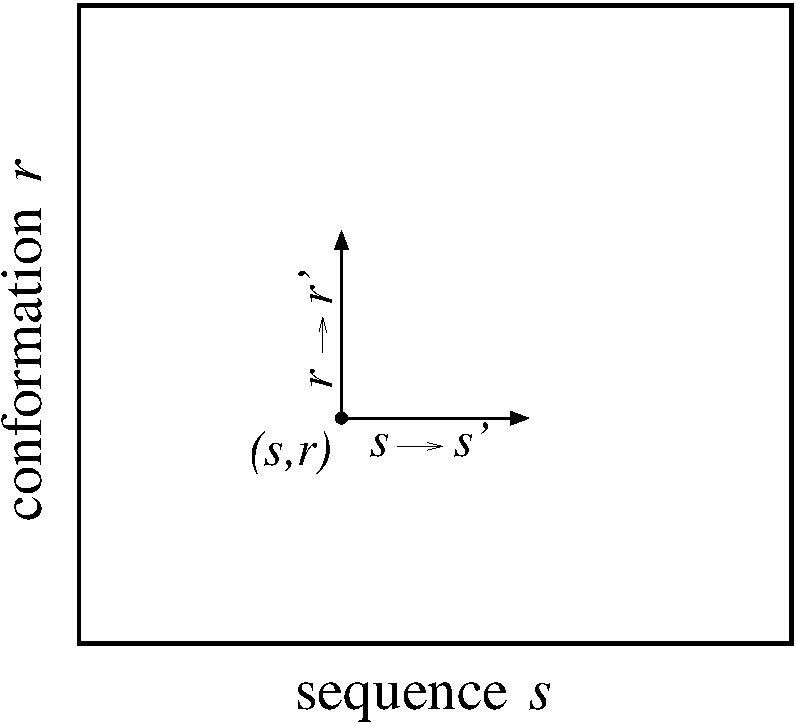
\includegraphics[width=4.2cm]{./Fig1}
\caption{The two types of Monte Carlo updates in the multisequence Monte Carlo algorithm.}
\end{figure}

\section{Theory}

\subsection{Generalized-ensemble algorithms and simulated tempering}

Conventional {\color{red} Metropolis} Monte Carlo simulations of the canonical distribution is problematic at low temperatures $T$ for many physical systems because simulations tend to become trapped in local energy minima and hamper representative sampling of configurational space. The basic idea of generalized-ensemble algorithms is to alleviate this trapping problem by sampling states using a non-Boltzmann weight factor and/or expand the state space with additional dynamical parameters~\cite{Mitsutake2001} {\color{red} (for a recent historical account see Ref.~\citenum{Berg2017}). Generalized-ensemble methods that have been frequently used for biomolecular simulations include simulated tempering (ST),~\cite{Marinari1992,Lyubartsev1992} replica exchange~\cite{Swendsen1986}  or parallel tempering,~\cite{Hansmann1997} and metadynamics.~\cite{Laio2002}}

ST is a direct extension to the Metropolis algorithm in which the temperature $T$ becomes a dynamic parameter. In this way, frequent visits to high $T$ allow simulations to readily escape from local energy minima. The algorithm thus simulates the joint probability distribution 
\begin{equation}
P(\rbar,m) =\dfrac{1}{\hat{Z}} e^{-\beta_m E(\rbar) + g_m}\,,
\label{ST}
\end{equation}
where  $\beta_m=1/k_\mathrm{B} T_m$, $\{T_m\}_{m=1}^\mathrm{M}$ a set of temperatures and $k_\mathrm{B}$ is Boltzmann's constant. The normalization constant in Eq.~\ref{ST} is  
\begin{equation}
\hat{Z} = \sum_r \sum_{m=1}^{\mathrm{M}}e^{-\beta_m E(\rbar) + g_m}\,,
\end{equation}
where the first sum is over all conformations $\rbar$. The simulation parameters $g_m$ control the marginal probability distribution
\begin{equation}
P(m) = \frac{1}{\hat{Z}}\sum_r e^{-\beta_m E(\rbar) + g_m} \,,
\end{equation}
and must therefore be carefully chosen. A common and convenient choice is $g_m\approx \beta_m F_m$, where $F_m$ is the free energy at temperature $T_m$. With this choice, $P(m)$ becomes approximately flat ensuring all temperatures are frequently visited. 

\subsection{Multisequence algorithm}
 
The basic idea of the MS algorithm for biomolecular simulation is to let the sequence $\sbar$ become a dynamic parameter rather than the temperature as in ST. A dynamic $\sbar$ is technically feasible when the potential energy can be written as $E(\sbar,\rbar)$, where $\sbar$ and $\rbar$ are independent variables. This is the case in our coarse-grained protein model which has only backbone degrees of freedom. It can also be achieved in some more detailed models.~\cite{Bhattacherjee2013,Wallin2017} 

Similarly to ST, the MS algorithm simulates the joint probability distribution
\begin{equation}
P(\sbar,\rbar) =\dfrac{1}{Z}e^{-\beta E(\sbar,\rbar) + h(\sbar)}\,, 
\label{MS}
\end{equation}
where  {\color{red}
\begin{equation}
Z = \sum_{\sbar\in\mathrm{S}}\sum_{\rbar} e^{-\beta E(\sbar,\rbar)+ h(\sbar)}\,
\label{eq:ZMS}
\end{equation}
and S is a set of pre-selected sequences, i.e., the sequences to which visits are allowed during a simulation.} The simulation parameters $h(\sbar)$, similar to the parameters $g_m$ in ST, control the marginal distribution $P(\sbar)=Z^{-1}\sum_{\rbar} e^{-\beta E(\sbar,\rbar)+ h(\sbar)} = \tilde{Z}^{-1}e^{-\beta F(\sbar)+ h(\sbar)}$ and a roughly flat $P(\sbar)$ can be achieved by choosing $h(\sbar) \approx \beta F(\sbar)$, where $F(\sbar)$ is the free energy of sequence $\sbar$ at temperature $T$. 

Two types of MC updates are required to sample from the distrubution in Eq.~\ref{MS}, ordinary conformational updates $\rbar\rightarrow\rbar'$ and {\color{red} sequence} updates $\sbar\rightarrow\sbar'$. The acceptance probabilities for the latter  becomes
\begin{equation}
P_\mathrm{acc} (\sbar\rightarrow\sbar') = \min [1, \exp\{-\beta\Delta E+\Delta h\}]\,,
\label{accrej}
\end{equation}
where $\Delta E = E(\sbar',\rbar)-E(\sbar,\rbar)$ and $\Delta h = h({\sbar'})-h(\sbar)$.

\section{Model and Methods}
\subsection{Coarse-grained 3-letter model for protein folding}

All calculations were carried out using the coarse-grained model for protein folding developed in Ref.~\citenum{Bhattacherjee2012}. In this model, there are 3 different amino acid types: hydrophobic (h), polar (p) and turn-type (t). The backbone chain is represented atomistically by the N, H, $\mathrm{C}_\alpha$, $\mathrm{H}_{\alpha 1}$, C$'$ and O atoms. By contrast, the sidechain represention is simplified to a single enlarged $\mathrm{C}_\beta$ atom, which is geometrically identical for h and p types. The sidechain is absent for the t type which instead has an $\mathrm{H}_{\alpha 2}$ atom. The t type is therefore closely related to glycine. All bond lengths, bond angles, and peptide plane angles (180$^\circ$) are held fixed. Hence, an $N$-amino acid chain conformation $\rbar$ can, for any sequence $\sbar$, therefore be described by the set of 2$N$ backbone torsional angles $\{\phi_i$, $\psi_i\}_{i=1}^{N}$. 
 
This geometrical description is paired with a simplified but finely tuned energy function with 4 terms: $E= E_\mathrm{ev} + E_\mathrm{loc} + E_\mathrm{hb} + E_\mathrm{hp}$. The first two, $E_\mathrm{ev}$ and $E_\mathrm{loc}$, represent excluded-volume effects and local electrostatic effects, respectively. The hydrogen-bond energy, $E_\mathrm{hb}$, represents directionally dependent interactions between NH and CO groups and is necessary for secondary structure formation. Finally, the ``hydrophobicity" term, $E_\mathrm{hp}$, implements pairwise Lennard-Jones-like interactions between the $C_\beta$ atoms of h amino acids which are necessary for driving chain collapse during folding. Various model parameters, e.g., the strengths of hydrophobic attractions and hydrogen bonding, were determined based on the ability of the model to spontaneously fold a set of model sequences with 18-54 amino acids into  structurally diverse and thermodynamically stable native states with both $\beta$ and $\alpha$-structure. As it turned out, this strategy made the model robust enough to fold sequences designed to have mixed $\alpha$ and $\beta$ structures. 

\subsection{Model sequences}

Six of the model sequences studied in this work, A1, N1, R1, R2, A2, and TN, are given in Table~I. In addition, we study two sequence sets $\mathrm{S16}_{1024}$  and $\mathrm{S35}_{1024}$ with 1,024 sequences each derived from the A1-N1 and A2-TN pairs, respectively, through mutational combinations, as well as the set $\mathrm{S16}_{144}$ taken from  Ref.~\protect\citenum{Holzgrafe2014}. 
 
\begin{table}
\caption{\label{tab1} List of 6 model sequences of different lengths $N$ studied in this work.}
\begin{ruledtabular}
\begin{tabular}{lcr}
Name & $N$ & Sequence \\
\hline
A1 & 16 & pphpphhpphpphhpp \\
N1 & 16 & phphphpttphphphp \\
R1 & 16 & pphhphptthpphhpp\\
R2 & 16 & ppphphhtthhphppp\\
A2 & 35 & (A1)ttt(A1)\\
TN & 35 & (A1)ttt(N1)\\
\end{tabular}
\end{ruledtabular}
\end{table}


\subsection{Monte Carlo simulation parameters and updates}

Both ST and MS simulations are carried out with two types of conformational updates $\rbar\rightarrow\rbar'$: (1) a global pivot move (20\%) which randomly picks a $\phi_\mathrm{i}$ angle or $\psi_\mathrm{i}$ angle and assign a new value between $-\pi$ and $\pi$; and (2) a semi-local move (80\%) which turns the $\phi_\mathrm{i}$ and $\psi_\mathrm{i}$-angles of 4 consecutive amino acids in a coordinated manner.~\cite{Favrin2001} 

%, and where S is the set of allowed (pre-selected) sequences, S (see Eq.~\ref{eq:ZMS})
%i.e., given by the $\phi_\mathrm{i}$ and $\psi_\mathrm{i}$ angles,

{\color{red}In MS simulations, sequence updates $\sbar\rightarrow\sbar'$ are carried out in the following way. First, a new random sequence $\sbar$ is picked from the set of pre-selected (allowed) sequences S, such that $\sbar'\ne\sbar$. The new sequence $\sbar'$ therefore differs from $\sbar$ in one or more amino acid positions. Thereafter, the sidechains of the protein, which remains in an unchanged (backbone) conformation $\rbar$, is re-built according to the new sequence $\sbar'$. Practically this means that, at the position(s) where the amino acid type has changed, the sidechain is altered according to the type change. For example, if $\mathrm{p}\rightarrow\mathrm{t}$, the $\mathrm{C}_\beta$ atom is removed and replaced with an $\mathrm{H}_{\alpha 2}$ atom or, if $\mathrm{p}\rightarrow\mathrm{h}$, the $\mathrm{C}_\beta$ remains in place but its character is changed to hydrophobic. Finally, the change in total energy $\Delta E$ is calculated and the accept-reject criterion in Eq.~\ref{accrej} is applied. If rejected, the old state $(\sbar,\rbar)$ is restored.} 

A sequence update is attempted every $1,000$ MC steps while temperature updates $m\rightarrow m'$ are attempted every 100 steps. {\color{red}The computational cost for sequence updates is somewhat higher than for temperature updates. The latter does not require any energy calculation and is thus extremely rapid. For the purpose of comparing computational efficiencies of ST and MS, we therefore chose sequence updates to be slightly less frequent than temperature updates while both are fairly frequent.} All simulations carried out in this work are summarized in Table~II.

\begin{table}
\caption{\label{tab2} List of simulations carried out in this work. }
\begin{ruledtabular}
\begin{tabular}{lcccr}
Runs & Algorithm & $\kb T$  & MC steps/run\footnote{Excludes a thermalization step with {\color{red} $10^7$} MC steps/run.} &  Sequences\\
\hline
32 & ST & 0.43--0.65 & $1\times10^7$ &A1\\ 
32 & ST & 0.43--0.65 & $1\times10^7$ &N1\\ 
32 & ST & 0.43--0.65 & $1\times10^7$ &R1\\ 
32 & ST & 0.43--0.65 & $1\times10^7$ &R2\\ 
32$\times$8\footnote{32 runs per temperature at 8 different temperatures.} & MS &0.43--0.65& $18\times 10^7$ & $\mathrm{S16}_{144}$\\
16 & MS & 0.43  & $5\times 10^9$ &  $\mathrm{S16}_{1024}$ \\
16 & MS & 0.46 & $4\times 10^9$ &  $\mathrm{S35}_{1024}$ \\
\end{tabular}
\end{ruledtabular}
\end{table}

\subsection{Observables}

Fold stabilities are calculated as in Ref.~\citenum{Holzgrafe2015} and described briefly below. First we define two structural similarity measures $\QIA$ and $\QIB$ for folds IA and IB, respectively, indicating the fraction of the fold-specific backbone-backbone hydrogen bonds that have been formed. The fold IA-hydrogen bonds are (2,6), (3,7), (4,8), (5,9), (6,10), (7,11), (8,12), (9,13), (10,14), (11,15) and the fold IB-bonds are (3,14), (5,12), (7,10), (10,7), (12,5), (14,3), where (i,j) indicates a hydrogen bond between the CO group of amino acid i and the NH group of amino acid j. The stabilities of folds IA and IB are defined as the probabilities $\PIA = P(\QIA\ge0.8)$ and $\PIB = P(\QIB\ge0.8)$, respectively, i.e., the probability that at least 80\% of the fold's hydrogen bonds are formed. $\PIA$ and $\PIB$ thus depend on both sequence $\sbar$ and temperature $T$. For example, $\PIA=0.875\pm 0.003$ for A1 and $\PIB=0.785\pm0.008$ for N1 at $\kb T = 0.43$. Structural similarity measures for 35-amino acid folds IIA and IIB are defined as $\QIIA = ( Q_\mathrm{IA}^\mathrm{1-16} + Q_\mathrm{IA}^\mathrm{20-35} + Q_\mathrm{tert} ) / 3$ and $\QIIB = ( Q_\mathrm{IA}^\mathrm{1-16} + Q_\mathrm{IB}^\mathrm{20-35} + Q_\mathrm{tert} ) / 3$, respectively, where superscripts on $\QIA$ and $\QIB$ indicate over which amino acid positions those measures are applied to within the longer 35 amino acid sequences and $Q_\mathrm{tert}$ is a measure that counts the number of $\mathrm{C}_\beta$-$\mathrm{C}_\beta$ contacts between the two secondary structure elements of these folds.~\cite{Holzgrafe2015} In analogy with $\PIA$ and $\PIB$, we define the stabilities of folds IIA and IIB as $\PIIA = P(\QIIA\ge0.8)$ and $\PIIB = P(\QIIB\ge0.8)$, respectively. The root-mean-square-deviation, RMSD, is calculated over all $\mathrm{C}_\alpha$ atoms.

\begin{figure}
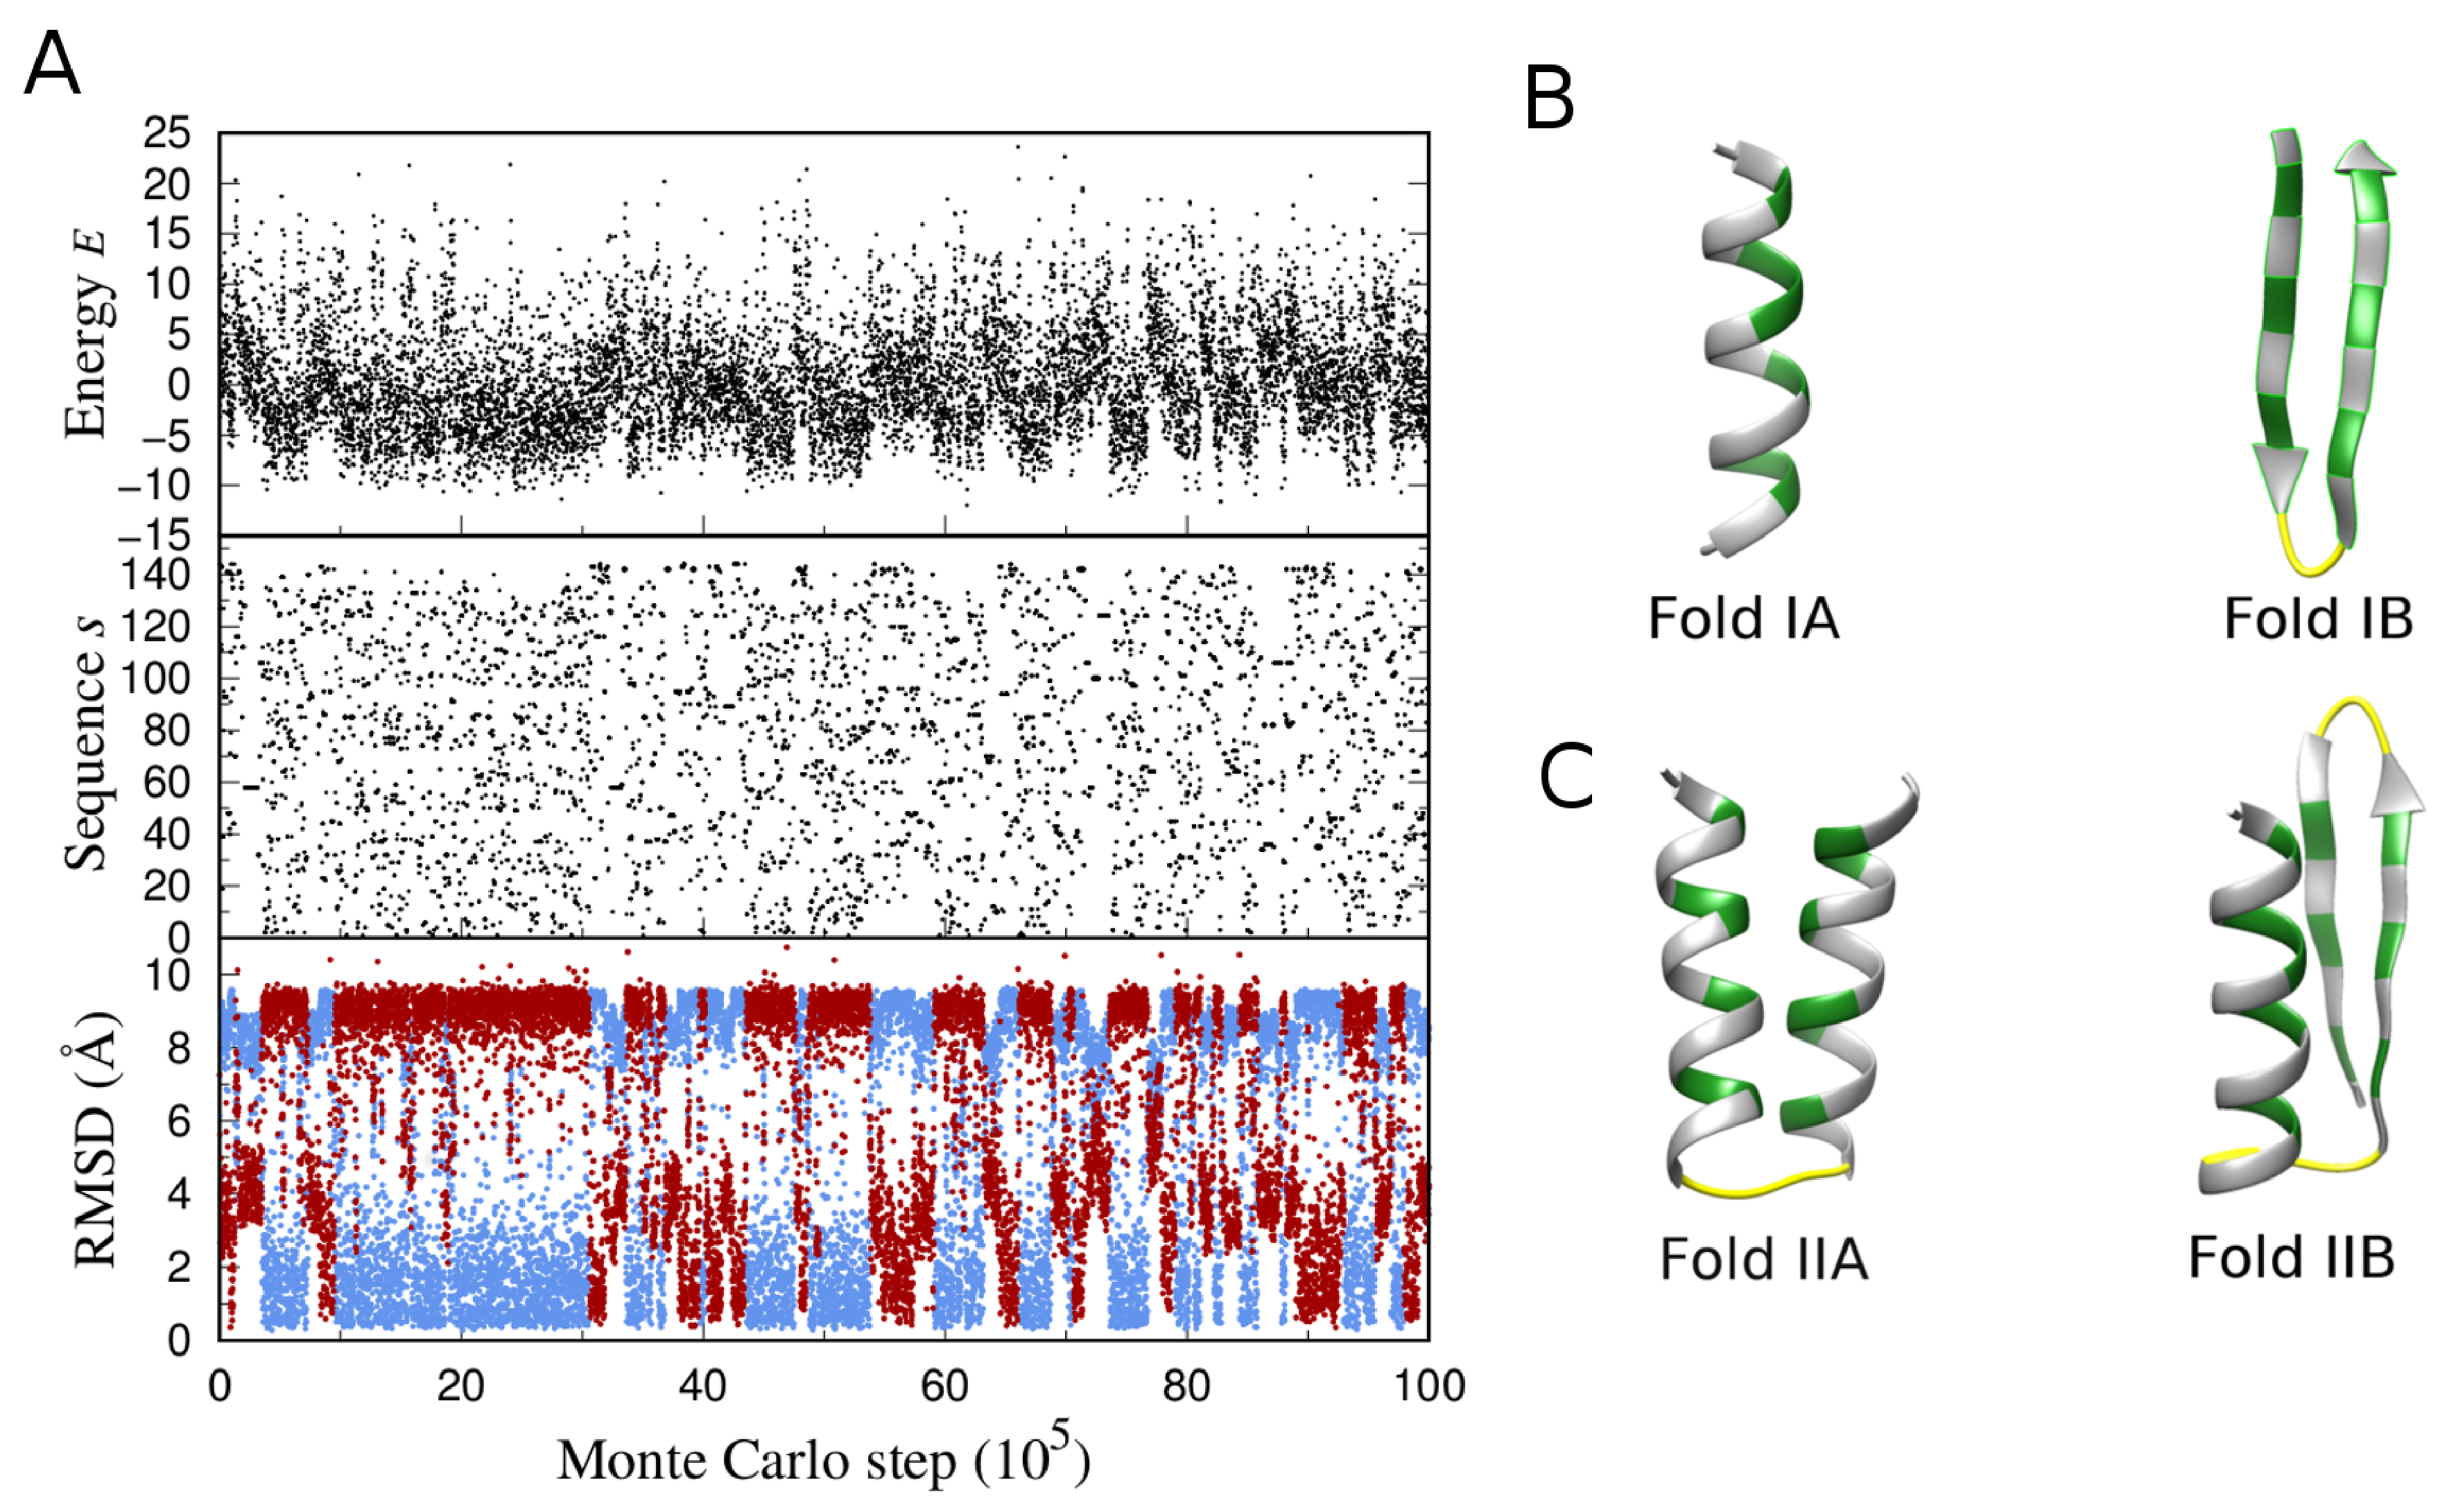
\includegraphics[width=8.5cm]{Fig2}
\caption{(A) Example of an MS simulation of the sequence set $\mathrm{S16}_{144}$ carried out at $\kb T = 0.43$. The plot shows the MC evolution of the sequence $\sbar$ (numbered 1--144), the total potential energy $E$ and the root-mean-square deviation (RMSD) calculated against the representative fold IA (light blue) and fold IB (dark red) structures in (B). Representative structures of folds (B) IA, IB, (C) IIA and IIB, chosen to be the minimum-energy conformations found for the sequences A1, N1, A2 and TN, respectively. }
\end{figure}

\section{Results}

\subsection{Computational efficiency}

We start by applying the MS algorithm to the set {\SR} across a range of temperatures $T$ (see Table~II). Two of the sequences in {\SR} are A1 and N1 (see Table~I) which fold into stable $\alpha$-helix and $\beta$-hairpin structures, respectively, as shown in Fig.~2B. Because A1 and N1 differ at 10 positions, 10 consecutive point mutations can transform A1 into N1, and vice versa. The binary sequence space between A1 and N1 in which any combination of these mutations have been carried out, therefore contains $2^{10}=1,024$ sequences. The 144 sequences in {\SR} were selected from this binary space with the constraints that the total number of hydrophobic amino acids are not too high and that they are not too unevenly distributed along the sequence.~\cite{Holzgrafe2014}

\begin{figure}
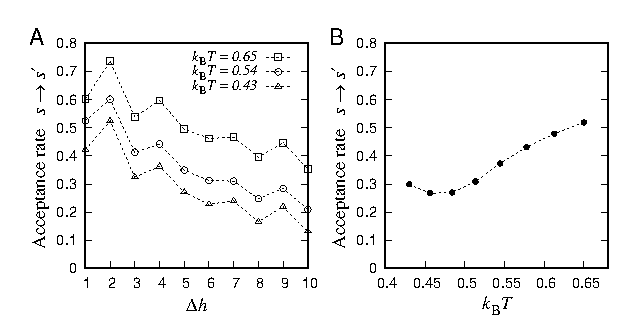
\includegraphics[width=7.8cm]{Fig3}
\caption{Acceptance rates for $\sbar\rightarrow\sbar'$ updates in MS simulations of the {\SR} sequence set as a function of (A) the number of changed amino acid positions $\Delta h$ and (B) temperature $T$. Acceptance rates for 3 different $T$'s are shown in (A).}
\end{figure}

Figure~2 illustrates a typical MS simulation trajectory carried out at the lowest studied temperature which is below the folding temperature of both A1 and N1.~\cite{Holzgrafe2014,Holzgrafe2015} From the MC evolution of the total energy $E$, sequence index $\sbar$, and RMSD values from the representative structures in Fig.~2B, it is evident that visits to various sequences drive transitions into a range of structural states. In particular, there are frequent visits to $\alpha$-helix and $\beta$-hairpin structures and transitions between them are accompanied by a shift in which sequences are preferably visited. For example, visits to high $\sbar$-indices, including N1 with index 144, tend to coincide with formation of $\beta$-hairpin structures as required to generate correct equilibrium conformational ensembles. 

One might have suspected that the MS algorithm would be hampered by poor acceptance rates for sequence updates. However, this is not the case in our model. We carry out updates $\sbar\rightarrow\sbar'$ by picking a new random sequence $\sbar'\ne\sbar$ from the set of allowed sequences. The (average) acceptance rate  depends on both $T$ and the step in sequences space $\Delta h$, i.e., the number of amino acid positions changed, as shown in Fig.~3. At the lowest $T$ and highest $\Delta h$, acceptance rates are only around 0.1-0.2. However, for most other $T$ and $\Delta h$ the overall acceptance rates are substantially higher and often above the oft-quoted rule-of-thumb value 0.25~\cite{Gilks1996} (see Fig~4B). An increased acceptance rate can easily be achieved by restricting proposed updates such that $\Delta h\le\Delta h_\mathrm{max}$, where $\Delta h_\mathrm{max}$ is a maximum step size, which might be necessary for longer chains. {\color{red} For example, $\Delta h_\mathrm{max} = 1$ would be equivalent to applying only a ``mutational" update, i.e., picking a random (allowed) position and changing the amino acid type at that position.}

\begin{figure}
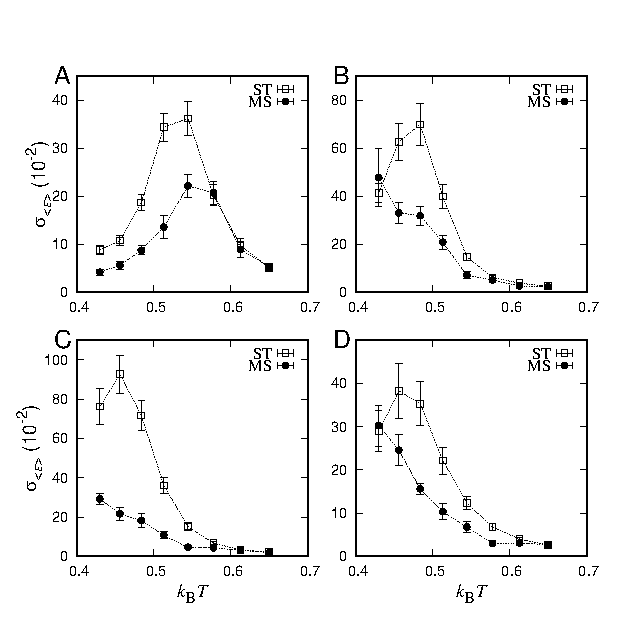
\includegraphics[width=8.0cm]{Fig4}
\caption{Comparing sampling efficiencies of the MS and ST algorithms. Statistical errors $\sigma_{\left < E\right >}$ of the average total energy $\left < E\right >$ obtained for the sequences (A) A1, (B) N1, (C) R1 and (D) R2 (see Table~I) at different temperatures $T$. Simulation lengths in the two methods are adjusted such that the number of conformations sampled per sequence and temperature is roughly the same (see text). }
\end{figure}

We now compare the results from our MS calculations with simulated tempering (ST) simulations carried out on 4 of the 144 sequences, namely A1 and N1 and two random sequences, R1 and R2, chosen at distances $h=4$ and $h=6$ from A1, respectively (see Table~I). While ST provides the thermodynamics of a given sequence across a range of $T$ in a single run, an MS simulation provides the thermodynamics of all 144 sequences at one $T$. We adjust the simulation lengths for ST and MS runs such that roughly the same number of sampled conformations are obtained for each $\sbar$ and $T$ combination, thus ensuring that similar computational resources are used for the two algorithms (see Table~II). We first validate the MS algorithm by comparing the average total energy, $\left < E \right >$, calculated for these 4 sequences with the two different methods (see Supplementary Information). The two sets of results are entirely consistent showing that, for a given $\sbar$ and $T$, the MS and ST algorithms indeed sample the same distribution. 

As a way to assess conformational sampling efficiency, we compare in Fig.~4 the statistical error, $\sigE$, of the average energy $\left <E\right >$ for the 4 sequences obtained using ST and MS, respectively. Because approximately the same number of sampled conformations were obtained for each combination of $\sbar$ and $T$, we compare the statistical errors directly. At the highest studied $T$, which is well above the folding temperature of both A1 and N1, the two algorithms give almost identical statistical errors. This can be understood by noting that at high-$T$ the free-energy landscape is relatively smooth and conformational space requires little difficulty to sample. The benefit of adding a dynamic parameter, whether $\sbar$ or $T$, is apparently minimal under these conditions. However, at lower $T$, the $\sigE$ values from MS is often smaller than those from ST and never significantly higher. For example, at the lowest $T$, the precision in the estimate of $\left < E\right >$ is roughly twice as high in MS than ST for A1 and R1, and roughly the same for N1 and R2. 

%The best estimate occurs at $\kb\approx$ 0.46 where MS is about 450\% better than ST. Even at the lowest T studied, MS is at least consistent or better than ST for all 4 sequences.


\begin{figure*}

\includegraphics[width=17.0cm]{Fig5}
\caption{Networks of sequences connecting folds IA and IB (top) and folds IIA and IIB (bottom). Each node represents a stable sequence ($\Ptot\ge\Pcut$ where $\Pcut=0.50$) that folds into either IA or IIA (light blue), IB or IIB (dark red), or is classified as bistable ($B>0.5$, black). A line between two nodes indicates that the sequences differ at only one position. Graph created using the tool Graphviz~\protect\cite{Graphviz2000} obtained from www.graphviz.org.}
\end{figure*}

\vspace{12pt}
\subsection{Exploring sequence space: IA/IB and IIA/IIB fold connectivities}

We now turn to the full binary sequence sets {\SI} and {\SII} with 1,024 sequences each. By applying the MS method to these two sets (see Table~II), we determine the low-$T$ thermodynamic behavior of each included sequence. In particular, we calculate the stabilities of folds IA and IB, $\PIA$ and $\PIB$, for all sequences in {\SI} and the stabilities of folds IIA and IIB, $\PIIA$ and $\PIIB$, for all sequences in {\SII} (see Methods). The relative statistical errors on these quantities vary but are only a few percent at the most, despite the large number of sequences included.  

Having calculated these fold stabilities, we are in a position to determine if there are pathways in sequence space that lead to abrupt IA-IB or IIA-IIB fold changes, i.e., paths that do not pass through any unstable intermediate sequence. To this end, we construct graphs in which each stable sequence is represented by a node and any two nodes are connected if their sequences differ at a single amino acid position. To determine if a sequence is stable we use the criterion $P_\mathrm{tot}>\Pcut$, where  $\Ptot = \PIA + \PIB$ and $\PIIA + \PIIB$ for the IA-IB and IIA-IIB fold pairs, respectively; $\Ptot$ thus indicates the total stability of a sequence across the two competing folds. The precise network depends, of course, on the cut-off value $\Pcut$ and a higher $\Pcut$ generally means a selection of more stable pathways. 

Fig.~5 illustrates the networks obtained with $\Pcut=0.50$ showing that both the IA-IB and IIA-IIB fold pairs are connected in sequence space at this stability threshold. A precise analysis shows that there are 516,972 viable IA-IB paths and 57,912 viable IIA-IIB paths. These paths represent 14.2 \% and 1.6 \% of all possible paths, respectively, because there are a total of $10! =3,628,800$ possible paths between start and end points in both cases. Hence, folds IA and IB are rather highly connected in our model for $\Pcut= 0.50$. For $\Pcut=0.60$, the numbers are 104,640 paths (2.9\%) for IA-IB and 22,512 (0.6\%) paths for IIA-IIB. We find that there are no possible IA-to-IB or IIA-to-IIB paths when $\Pcut\ge0.74$ and $\ge 0.66$, respectively. \\

\subsection{Biophysical properties of fold-to-fold mutational pathways}
 
An apparently general characteristic of designed and natural proteins that exhibit mutation-induced fold switching is a reduced stability near the switch point.~\cite{Alexander2009,He2012,Kouza2012,Sikosek2016,Sutto2012} Our model proteins exhibit a similar trend. Fig.~6A and B show the average total stability $\Ptot$ for sequences found at different Hamming distances $h$ from the starting point. Intermediate sequences are less stable than sequences at distances $h=0$ (A1 or A2) and $h=10$ (N1 or TN), although there are large variations between sequences as indicated by the upper and lower bounds. There is nonetheless a clear statistical trend that sequences become gradually less stable as successive mutations are applied to any of the 4 start and end points until a minimum is reached. 
%These minima in stability occur closer to N1 and TN in the two systems, respectively, indicating that the IA/IIA folds are more mutationally robust than the IB/IIB folds. 

\begin{figure}
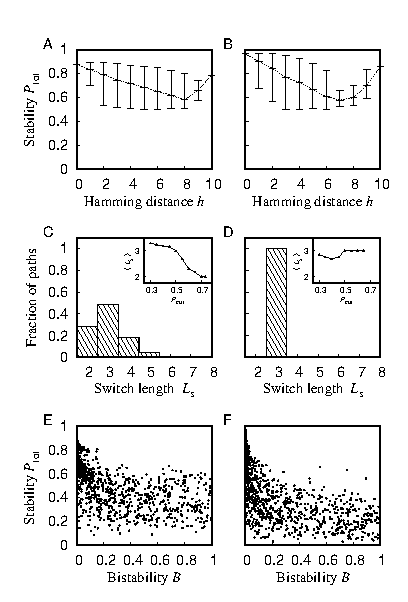
\includegraphics[width=7.8cm]{Fig6}
\caption{Stability properties of mutational pathways. The total stability $\Ptot$ as a function of the distance $h$ from A1 averaged over all (A) IA-IB and (B) IIA-IIB mutational paths obtained with $\Pcut=0.50$. Error bars indicate maximum and minimum $\Ptot$ values. The distribution of switch lengths $L_\mathrm{s}$ for the (C) IA-IB and (D) IIA-IIB mutational paths ($\Pcut=0.50$). C and D insets: Average switch length $\left < L_\mathrm{s}\right >$ across all paths as a function of $\Pcut$. Scatter plots of $\Ptot$ versus bistability $B$ for all sequences in (E) {\SI} and (F) {\SII}, where $B=1-\Delta P/\Ptot$ and $\Delta P = |\PIA-\PIB|$ or $|\PIIA-\PIIB|$.}
\end{figure}

%The smooth average stability trends in Fig.~6 might have been underpinned by individual mutational pathways that gradually shift the population between the two folds, however, this is not the case.

However, the smooth stability trends in Fig.~6A and B belie the real character of the individual mutational pathways which tend to exhibit an abrupt switch between the two folds. To see this and to further examine the character of the fold transitions in our model, we make a distinction between two types of stable sequences: those that fold into a single unique fold, thus behaving as classical proteins, and those that display substantial stabilities of both folds. Such ``bistable" sequences are interesting from a biophysical perspective in that they are able to fold into two alternative folds. Indeed, bistable sequences have been proposed to play a role in the evolution of new protein folds.~\cite{Sikosek2012} We consider a sequence to be bistable if $B>0.5$, where $B$ is a bistability measure (see Fig.~6 legend). In principle, a fold transition can then occur directly between two classical proteins with unique native folds, or it can proceed via one or more intermediate bistable sequences which populate both folds. We define the switch length of a mutational pathway $L_\mathrm{s}=2+n_\mathrm{B}$, where $n_\mathrm{B}$ is the number of bistable sequences in between the two classical sequences that define the switch point. Hence, a path with $L_\mathrm{s}=2$ accomplishes a fold switch in a single mutational step without going through a bistable point. From the distributions of  $L_\mathrm{s}$ in Fig.~5C and D, taken over all pathways with $\Pcut=0.50$, it can be seen that fold switching along individual pathways are typically completed in only 1-2 mutations and a single step is often sufficient to switch between the IA and IB folds. Hence, fold switching is typically abrupt and, for $\Pcut = 0.5$, it is fairly common that viable pathways pass through one or two bistable sequences. 

Interestingly, switching between folds IA and IB through one or more bistable sequences become less and less frequent as selections for more stable pathways are made. This can be seen from the decrease in $\left <L_\mathrm{s}\right >$ as a function of $\Pcut$ (see Fig.~5C(inset)). For $\Pcut\ge0.70$, there are no longer any remaining path between the $\alpha$-helix and $\beta$-hairpin that passes through a bistable sequence because $\left <L_\mathrm{s}\right > =  2$. An underlying reason for the occurrence of sharper fold switches for more stable mutational pathways is apparent from a comparison between $\Ptot$ and $B$ across all sequences in {\SI}. As shown in Fig.~5E, sequences with the highest $\Ptot$ tend to exhibit very little bistability. Hence, highly stable paths are therefore forced to go through abrupt switch points where they transition directly between folds in a single step. The situation for the IIA-IIB fold pair is more complicated. We find that, just as for {\SI}, sequences in {\SII} follow the trend that the highest $\Ptot$ values occur for only classical, low-$B$ proteins. One might therefore expect that selection of more stable IIA-IIB paths would decrease $\left <L_\mathrm{s}\right >$, however, this is not the case as such abrupt switch points between the IIA and IIB are not available for $\Pcut\ge0.50$ (cf. Fig.~5 bottom). As a result, bistable sequences do play a crucial role in bridging the IIA and IIB folds, although passing though these sequences lead to additional reduction in stability at the switch point. 
 
\section{Discussion}

We have evaluated a biomolecular simulation algorithm that works by making the biological sequence a dynamic parameter. As a test, we applied it on a CG model for protein folding. The results indicate that there are two main benefits of this approach. Firstly, it provides a convenient way to sample the canonical distributions of large numbers of sequences in a single run and, secondly, it enhances the sampling of conformational space meaning it can be applied directly at low temperatures. The conformational sampling efficiency can be assessed from the comparison with ST. Although there is no single ``fair" way to compare the two methods, we chose as a measure of efficiency the statistical error of the total energy, $\sigE$, obtained with roughly the same computational cost per temperature and sequence. At the highest studied temperatures, we find that the statistical errors $\sigE$ are basically the same. This finding is not unexpected because conformational sampling of short polymers at high $T$ does not involve crossing any major energy barriers. As a result, successively sampled conformations for a given combination of sequence $\sbar$ and temperature $T$, are likely uncorrelated in both methods which leads to similar $\sigE$ values. 

At lower temperatures, we find that the MS simulations often yields significantly smaller $\sigE$ than ST simulations. It is notable that this acceleration in conformational sampling vis-{\'a}-vis ST is achieved despite that simulations are carried out at constant $T$. {\color{red} Therefore, rather than promoting escape from local minima by visits to higher $T$, as in  ST~\cite{Marinari1992,Lyubartsev1992} or temperature replica-exchange,~\cite{Swendsen1986} MS simulations must escape the minima occurring for one sequence through visits to other sequences. How this process works can be envisioned by considering an MS simulation that is visiting a sequence $s$ and is trapped in a local minimum, requiring that a high free-energy barrier is overcome for escape. The trapped state could be, e.g., a compact $\beta$-sheet rich state with a particular register. Eventually, sequence updates will carry the simulation to other sequences $\hat{s}$ while still remaining in the trapped state. However, the free energy barrier of this trapped state might be substantially lower for $\hat{s}$ than for $s$, or the barrier may even be altogether absent if the trapped state is unstable for $\hat{s}$, leading to rapid escape from the minimum. } The above reasoning also implies that the performance of the MS algorithm likely depends on the size the sequence set S as well as the conformational properties of the sequences. Specifically, the performance of MS simulations of proteins at low $T$ may benefit from the inclusion of at least a few sequences with poor stability properties, such that partial unfolding of the chain is regularly triggered and thus promoting transitions to new conformational states. 

{\color{red} Individual protein sequences that exhibit spontaneous transitions between widely different competing conformational states, such as fold switching proteins, are especially challenging to molecular simulation methods. This problem has been addressed by using Hamiltonian replica-exchange techniques to couple G\={o}-like terms, i.e., energy terms with an artificial bias towards a given structure, with a physical force field.~\cite{Meinke2007,Chen2014,Bernhardt2016} This way exchange moves ``feed" conformations into the replica corresponding to the physical force field and enhance sampling.~\cite{Bernhardt2016} We did not specifically study sampling efficiency for sequences exhibiting competing states. It appears likely, however, that a very similar type of ``feeding" of conformations would take place in MS simulations although the coupling occurs instead with other sequences rather than with G\={o}-type terms. }

We emphasize that the MS method should not be seen as a general technique to speed up conformational sampling. However, our results indicate that for CG models that permit sequence updates to be carried out as a simple Metropolis step and when visits to higher $T$ is unwanted (or unnecessary), our method can be a highly efficient way to sample the equilibrium behavior of many sequences. {\color{red} This opens up for various applications, such as exploring sequence effects on the conformational properties of disordered~\cite{Das2013} or denatured~\cite{Meng2013} proteins, or as a tool in efforts to combine population genetics and molecular simulations.~\cite{Serohijos2014} While applied to proteins in this work, we note that the MS algorithm is equally valid for other bio-macromolecules, including DNA and RNA.} The ability to promote conformational sampling without resorting to an increase in $T$ may make the method useful in simulations of biomolecules in ordered phases, such as lipid bilayers or double-stranded DNA, where escape from local minima can be especially challenging~\cite{Bereau2015,Curuksu2009} and elevated $T$ is typically avoided in simulations because it may lead to unwanted perturbations or unfolding of the basic underlying structure.

\section{Conclusion}

We have evaluated an algorithm for biomolecular simulations that allows the thermodynamics of multiple  sequences to be calculated in a single run. We applied the algorithm to protein folding and showed that the thermodynamic behavior of $>$1,000 amino acid sequences with up to 35 amino acids could be determined in an intermediate-resolution CG model. The method performs a random walk in sequence space which is especially useful at low temperature as it promotes escape from local minima present in the free energy landscapes of individual sequences. The method might be suitable for CG simulations of {\color{red} various} other biomolecular systems, such as peptides in phospholipid bilayers, where sampling at elevated temperatures is not desirable. 

\section{Supplementary Materia} 

Validation of the MS algorithm. 

\section{Acknowledgments}

This work was supported by grants from Memorial University and National Sciences and Engineering Research Council of Canada (RGPIN-2016-05014).  

\bibliography{/Users/stefan/Documents/Manuscripts/Jshort,/Users/stefan/Documents/Manuscripts/MyRefs}
%% ****** Start of file aipsamp.tex ******
%
%   This file is part of the AIP files in the AIP distribution for REVTeX 4.
%   Version 4.1 of REVTeX, October 2009
%
%   Copyright (c) 2009 American Institute of Physics.
%
%   See the AIP README file for restrictions and more information.
%
% TeX'ing this file requires that you have AMS-LaTeX 2.0 installed
% as well as the rest of the prerequisites for REVTeX 4.1
%
% It also requires running BibTeX. The commands are as follows:
%
%  1)  latex  aipsamp
%  2)  bibtex aipsamp
%  3)  latex  aipsamp
%  4)  latex  aipsamp
%
% Use this file as a source of example code for your aip document.
% Use the file aiptemplate.tex as a template for your document.
\documentclass[%
 aip,
%jmp,%
%bmf,%
%sd,%
rsi,%
 amsmath,amssymb,
%preprint,%
 reprint,%
%author-year,%
%author-numerical,%
]{revtex4-1}

\usepackage{graphicx}% Include figure files
\usepackage{dcolumn}% Align table columns on decimal point
\usepackage{bm}% bold math
%\usepackage[mathlines]{lineno}% Enable numbering of text and display math
%\linenumbers\relax % Commence numbering lines

\newcommand	 {\sbar}	{{s}}
\newcommand	 {\rbar}	{{r}}
\newcommand	 {\hi}		{{h_\mathrm{i}}}
\newcommand	 {\pii}  	{{p_\mathrm{i}}}
\newcommand	 {\kb}		{{k_\mathrm{B}}}
\newcommand	 {\Tlow}	{{T_\mathrm{low}}}
\newcommand 	 {\Pnat} 	{{P_\mathrm{nat}}}
\newcommand {\Qa}		{{Q_\mathrm{A}}}
\newcommand {\Qb}		{{Q_\mathrm{B}}}
\newcommand {\Pcut}     	{{P_\mathrm{cut}}}
\newcommand {\TlowI}     {{T^\mathrm{I}_\mathrm{low}}}
\newcommand {\TlowII}    {{T^\mathrm{II}_\mathrm{low}}}
\newcommand {\Ptot}	{{P_\mathrm{tot}}}
\newcommand {\PaI}    	{{P_\mathrm{IA}}}
\newcommand {\PbI}    	{{P_\mathrm{IB}}}
\newcommand {\PaII}    	{{P_\mathrm{IIA}}}
\newcommand {\PbII}    	{{P_\mathrm{IIB}}}
\newcommand {\SR}		{{S144}}
\newcommand {\SI}		{{SBI}}
\newcommand {\SII}		{{SBII}}

\begin{document}

\preprint{AIP/123-QED}

\title[Multisequence Monte Carlo simulations]{Exploring mutation-induced protein fold switching using multisequence Monte Carlo simulations}

\author{A. Aina}
\author{S. Wallin}
\email{swallin@mun.ca}
\affiliation{ 
Memorial University of Newfoundland, Department of Physics and Physical Oceanography, A1B 3X7 St John's, NL, Canada}

\date{\today}

\begin{abstract}
We test an algorithm that can calculate the thermodynamic behavior of multiple amino acid  sequences in a single enhanced Monte Carlo run, in a coarse-grained protein model. 
\end{abstract}

\pacs{Add  here}
                             
\keywords{Generalized-ensemble algorithm, simulated tempering, protein folding, protein fold switching, coarse-grained model}


\maketitle

\section{Introduction}
\noindent
Modern investigations into biophysical properties of biomolecular systems are routinely carried out not only on a single species but on multiple molecular variants.~\cite{Vukmirovic2000,Nickson2010} For example, protein engineering methods are used to provide mechanistic insight into the specificity of protein-protein and protein-DNA interactions, to compare the  conformational propensities of disease-related mutations of aggregation-prone proteins, and optimize biomolecular properties through directed evolution. Moreover, large-scale screening techniques such as phage display and microarray chips are used to provide biophysical properties across entire genomes. In short, through the study of a biomolecular system and related variants molecular variants are studied in order to gain a more complete picture of the biophysical and biochemical properties of the system and provide evolutionary context. 

While protein or DNA sequences are easily changed on the computer, the high computational cost of simulating even a single moderately-sized biomolecule makes systematic explorations of sequence space challenging. Some notable efforts have nonetheless been attempted, including simulations of all 136 unique tetranucleotide sequences in B-DNA oligonucleotides using all-atom explicit water molecular dynamics.~\cite{Beveridge2004}

Here we explore a Monte Carlo (MC)-based algorithm for calculating the folding thermodynamics of multiple protein sequences in a single enhanced run. The algorithm relies on sampling at fixed temperature a generalized ensemble in which the sequence is treated as a dynamic parameter. Hence, this multisequence MC method includes two main types of updates: conformational updates $\rbar\rightarrow\rbar'$ and sequences updates $\sbar\rightarrow\sbar'$. As illustrated in Fig.~1, this approach requires that $\rbar$ and $\sbar$ are ``perpendicular" coordinates such that the potential energy of the model can be written in terms of two independent variables, $E(\sbar,\rbar)$. While this may be hard to achieve for detailed protein models, it is likely possible for many coarse-grained models. 

We first apply the MS algorithm to a set of 144 model sequences with 16 amino acids and compare with the simulated tempering (ST) algorithm. We find that the computational efficiency of the MS algorithm is never less efficient than ST even at the lowest studied temperature. The model folds spontaneously designed sequences into stable native states with diverse protein-like sequences, and captures features such as mutational robustness. It therefore provide a biophysical basis for the sequence-structure and sequence-stability relationships of proteins at a conceptual level. This model has been used, e.g., to study the sequence-structure relationship of proteins in the "marshlands" between protein folds. Experimental studies have indicated that single point mutations are capable to take change one protein fold into another. The multisequence algorithm allow us to characterize the stability of and structure of all 1,024 sequence in the binary space between the two folds. The implication of these results for the fold switching and evolution is discussed. \\

We then demonstrate that the multisequence algorithm can be used to calculate the thermodynamic behavior for $>1,000$ sequences in a 3-letter model for protein folding~\cite{Bhattacherjee2012} at temperatures well below the typical folding temperatures $T_\mathrm{f}$ of the included sequences.  

While the 16-amino acid A1 and N1 sequences fold into $\alpha$-helical and $\beta$-hairpin folds, respectively, the two 35-amino acid sequences A2 and TA adopt the folds denoted IIA and IIB, as shown in Fig.~X. 

The large number of sequences considered allows us to carry out a much more systematic analysis than previously~\cite{Holzgrafe2014,Holzgrafe2015} of the sequence-structure-stability relationship in the sequence region that connect these two folds pairs. We find that...


\begin{figure}
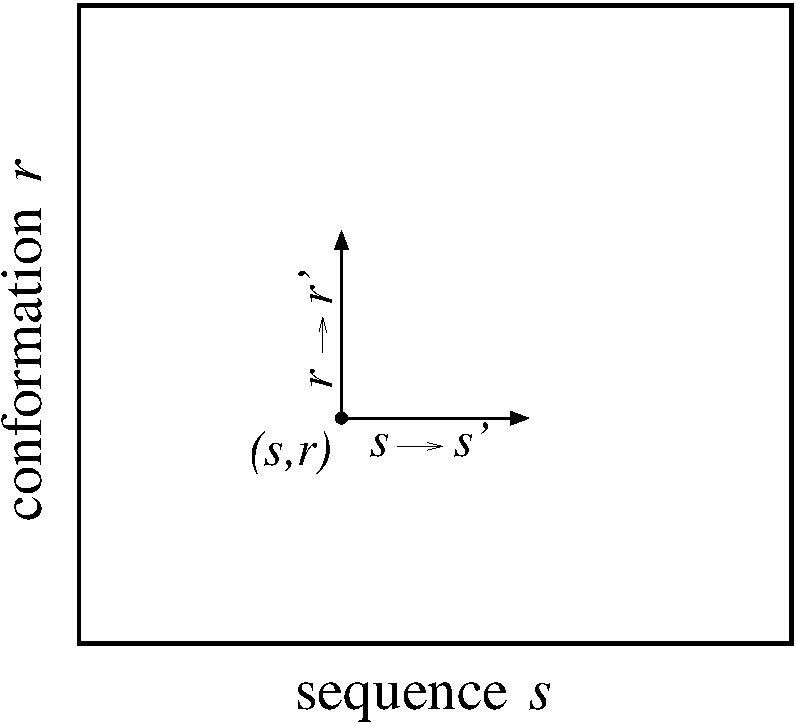
\includegraphics[width=4.2cm]{Fig1}
\caption{The two types of Monte Carlo updates in the multisequence Monte Carlo algorithm.}
\end{figure}

\section{Theory}

\subsection{Generalized-ensemble algorithms and simulated tempering}
\noindent
Conventional Monte Carlo simulations of the canonical distribution is problematic at low temperatures $T$ for many physical systems because simulations tend to become trapped in local energy energy minima and hamper representative sampling of configurational space. The basic idea of generalized-ensemble algorithms~\cite{Mitsutake2001} is to alleviate this trapping problem by sampling states using a non-Boltzmann weight factor and/or expand the state space with additional dynamical parameters, such that a more efficient random walk in potential energy can be achieved. 

A well-known generalized-ensemble algorithm is simulated tempering (ST),~\cite{Marinari1992,Lyubartsev1992} in which it is the temperature $T$ that becomes a dynamic parameter. In this scheme, frequent visits to high-$T$ allow simulations to readily escape from local energy traps. The ST algorithm thus simulates the joint probability distribution 
\begin{equation}
P(\rbar,m) =\dfrac{1}{\hat{Z}} e^{-\beta_m E(\rbar) + g_m}\,,
\label{ST}
\end{equation}
where  $\beta_m=1/k_\mathrm{B} T_m$, $\{T_m\}_{m=1}^\mathrm{M}$ a set of temperatures and $k_\mathrm{B}$ is Boltzmann's constant. The normalization constant in Eq.~\ref{ST} is  
\begin{equation}
\hat{Z} = \sum_r \sum_{m=1}^{\mathrm{M}}e^{-\beta_m E(\rbar) + g_m}\,,
\end{equation}
where the first sum is over all conformations $\rbar$. The simulation parameters $g_m$ control the marginal probability distribution
\begin{equation}
P(k) = \frac{1}{\hat{Z}}\sum_r e^{-\beta_m E(\rbar) + g_m} \,,
\end{equation}
and must therefore be carefully chosen. A common and convenient choice is $g_m\approx \beta_m F_m$, where $F_m$ is the free energy at temperature $T_m$. With this choice, $P(k)$ becomes approximately flat ensuring all temperatures are frequently visited. 

\subsection{Multisequence algorithm}
\noindent 
The basic idea of the MS algorithm for biomolecular simulation is to let the sequence $\sbar$ become a dynamic parameter rather than the temperature as in ST. A dynamic $\sbar$ is technically feasible as long as the potential energy can be written as $E(\sbar,\rbar)$, where $\sbar$ and $\rbar$ are independent variables. This is the case in our coarse-grained protein model with only backbone degrees of freedom and can also be achieved for more detailed  models~\cite{Bhattacherjee2013,Wallin2017}. 

In analogy with ST, the MS algorithm simulates the joint probability distribution
\begin{equation}
P(\sbar,\rbar) =\dfrac{1}{\tilde{Z}}e^{-\beta E(\sbar,\rbar) + h(\sbar)}\,, 
\label{MS}
\end{equation}
where  
\begin{equation}
\tilde{Z} = \sum_{\sbar}\sum_{\rbar} e^{-\beta E(\sbar,\rbar)+ h(\sbar)}\,
\end{equation}
and the first sum goes over a set of allowed sequences $\sbar$. The simulation parameters $h(\sbar)$, similarly to the parameters $g_m$ in ST, control the marginal distribution $P(\sbar)=\tilde{Z}^{-1}\sum_{\rbar} e^{-\beta E(\sbar,\rbar)+ h(\sbar)} = \tilde{Z}^{-1}e^{-\beta F(\sbar)+ h(\sbar)}$ and a roughly flat $P(\sbar)$ can be achieved by choosing $h(\sbar) \approx \beta F(\sbar)$, where $F(\sbar)$ is the free energy of sequence $\sbar$ at temperature $T$. 

Two types of MC updates are required to sample from the distrubution in Eq.~\ref{MS}, ordinary conformational update $\rbar\rightarrow\rbar'$ and mutational updates $\sbar\rightarrow\sbar'$. The acceptance probabilities for the latter  becomes
\begin{equation}
P_\mathrm{acc} (\sbar\rightarrow\sbar') = \min [1, \exp\{-\beta\Delta E+\Delta h\}]\,,
\label{accrej}
\end{equation}
where $\Delta E = E(\sbar',\rbar)-E(\sbar,\rbar)$ and $\Delta h = h_{\sbar'}-h(\sbar)$.

\section{Methods}
\subsection{Coarse-grained 3-letter model for protein folding}
\noindent
All calculations were carried out on a coarse-grained model for protein folding~\citenum{Bhattacherjee2012}. In this model, there are 3 different amino acid types: hydrophobic (h), polar (p) and turn-type (t). The backbone chain is represented atomistically by the N, H, $\mathrm{C}_\alpha$, $\mathrm{H}_{\alpha 1}$, C$'$ and O atoms. By contrast, the sidechain represention is simplified to a single enlarged $\mathrm{C}_\beta$ atom, which is geometrically identical for h and p types. The sidechain is absent for the t type which instead has an $\mathrm{H}_{\alpha 2}$ atom. The t type is therefore closely related to glycine. All bond lengths, bond angles, and peptide plane angles (180$^\circ$) are held fixed. Hence, an $N$-amino acid chain conformation $\rbar$ can, for any sequence $\sbar$, is therefore described by the set of 2$N$ backbone torsional angles $\{\phi_i$, $\psi_i\}_{i=1}^{N}$. 
 
This geometrical description is paired with a simplified but finely tuned energy function with 4 terms: $E= E_\mathrm{ev} + E_\mathrm{loc} + E_\mathrm{hb} + E_\mathrm{hp}$. The first two, $E_\mathrm{ev}$ and $E_\mathrm{loc}$, represent excluded-volume effects of all atoms and local electrostatic effects, respectively. The hydrogen-bond energy, $E_\mathrm{hb}$, represents directionally dependent interactions between NH and CO groups which are necessary for secondary structure formation. Finally, the ``hydrophobicity" term, $E_\mathrm{hp}$, implements pairwise Lennard-Jones-like interactions between the $C_\beta$ atoms of h amino acids which are necessary for driving chain collapse during folding. Various model parameters, e.g., the strengths of hydrophobic attractions and hydrogen bonding, were determined based on the ability of the model to spontaneously fold a set of model sequences with 18-54 amino acids into  structurally diverse and thermodynamically stable native states with both $\beta$ and $\alpha$-structure. As it turned out, this strategy made the model robust enough to fold sequences designed to have mised $\alpha$ and $\beta$ structure. 
 
\subsection{Sequence sets}
\noindent


\begin{table}
\caption{\label{tab:table1} Model sequences of different sequence lengths $N$ studied in this work. In addition to the 6 sequences listed, we studied sets of 1,024 sequences derived from the A1-N1 and A2-TN pairs, respectively, (see text) denoted S16 and S35, respectively, and a restricted S16-set of 144 sequences denoted $\mathrm{S16}_{144}$ (also studied in Ref.~\protect\citep{Holzgrafe2014}).  }
\begin{ruledtabular}
\begin{tabular}{lcr}
Name & $N$ & Sequence\\
\hline
N1 & 16 & phphphpttphphphp \\
A1 & 16 & pphpphhpphpphhpp \\
Ran1 & 16 & \textbf{(add)}\\
Ran2 & 16 &  \textbf{(add)}\\
A2 & 35 & A1-ttt-A1\\
TN & 35 & A1-ttt-N1\\
\end{tabular}
\end{ruledtabular}
\end{table}


\subsection{Monte Carlo simulation parameters}
\noindent
Both ST and MS simulations are carried out with two types of conformational updates $\rbar\rightarrow\rbar'$: (1) a global pivot move (20\%) which randomly picks a $\phi_\mathrm{i}$ angle or $\psi_\mathrm{i}$ angle and assigned a new value between $-\pi$ and $\pi$; and (2) an approximately local move (80\%) which turns the $\phi_\mathrm{i}$ and $\psi_\mathrm{i}$-angles of 4 consecutive amino acids in a coordinated manner.~\cite{Favrin2003} In MS simulations, sequence updates $\sbar\rightarrow\sbar'$ are attempted every $1000$ step and carried out by randomly picking a new sequence $\sbar'\ne\sbar$ and applying the accept-reject criterion in Eq.~\ref{accrej}. In ST, temperature updates $m\rightarrow m'$ are attempted every 100 steps. Observables are sampled every 10 or 100 MC step. All simulations carried out in this work are summarized in Table~1. 

\begin{table}
\caption{\label{tab:table1} List of simulations carried out in this work. }
\begin{ruledtabular}
\begin{tabular}{lccccr}
Runs & Algorithm & $T$ & MC steps &  Sequence set\\
\hline
32$\times$4\footnote{32 runs carried out for each of the 4 sequences. } & ST & $8\times 10^6$ &A1,N1,Ran1,Ran3\\
32$\times$8\footnote{32 independent runs carried out at each of the temperatures $T_1$ to $T_8$} & MS & $144\times 10^6$ & 16 &$\mathrm{S16}_{144}$\\
16 & MS & $5\times 10^9$ & 16 & S16 \\
16 & MS & $4\times 10^9$ & 35 & S35 \\
\end{tabular}
\end{ruledtabular}
\end{table}

\subsection{Stability measures}
\noindent
To quantify the stabilities of various folds, we use the measures used in Ref.~\cite{Holzgrafe2015}. We classify conformations $r$ as part of a fold if $Q\ge0.8$ where $Q\in [0,1]$ quantifies the similarity of $r$ to that fold. For folds A and B, $Q$ is determined by defining a set of backbone-backbone hydrogen bonds that are present in those folds (ignoring N and C terminal amino acids). For fold A, the fold-specific set of contacts (i,j) between the CO group of amino acid i and the NH group of amino acid j is $\{$(2,6), (3,7), (4,8), (5,9), (6,10), (7,11), (8,12), (9,13), (10,14), (11,15)$\}$, and for fold B the contact set is $\{$(3,14), (5,12), (7,10), (10,7), (12,5), (14,3)$\}$. A hydrogen bond is considered formed if (i) the NHO and COH angles both are $>90^\circ$ and (ii) the HO distance is $<2.7$~{\AA}. 

%\begin{equation}
%Q_\mathrm{2\alpha} = ( Q_\alpha^\mathrm{1-16} + Q_\alpha^\mathrm{20-35} + Q_\mathrm{tert}) ) / 3
%\end{equation}
%
%\begin{equation}
%Q_\mathrm{\alpha\beta} = ( Q_\alpha^\mathrm{1-16} + Q_\beta^\mathrm{20-35} + Q_\mathrm{tert} ) / 3
%\end{equation}

\begin{figure}
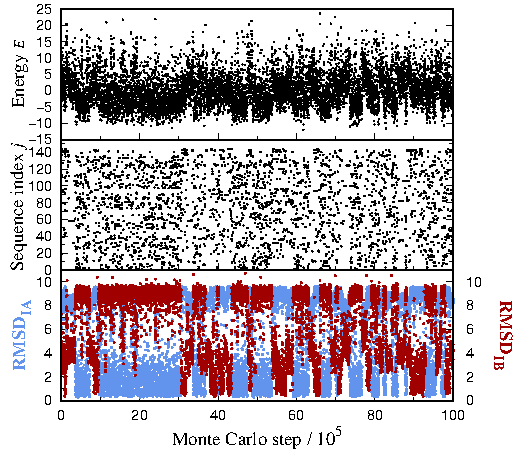
\includegraphics[width=6.0cm]{MCtraj}
\caption{Example of a multisequence simulation.}
\end{figure}

%
%\begin{equation}
%Q_\mathrm{\alpha\beta\beta} = ( Q_\alpha^\mathrm{1-12} + Q_\beta^\mathrm{XX} +Q_\beta^\mathrm{20-35} + Q_\mathrm{tert} ) / 4
%\end{equation}
%
%
%\begin{equation}
%Q^*_\mathrm{\alpha\beta} = [ \max(Q_\alpha^\mathrm{1-16},Q_\beta^\mathrm{XX}) +Q_\beta^\mathrm{20-35} + Q_\mathrm{tert}) ] / 3
%\end{equation}
%

\section{Results}

\subsection{Computational efficiency of the multisequence algorithm}
\noindent
To assess the computational efficiency and properties of the multisequence algorithm, we used as a test case the set of 144 3-letter model sequences with 16 amino acids studied in Refs.\cite{Holzgrafe2014} Two of the sequences are A1 and N1 which were designed to fold into stable $\alpha$-helix and $\beta$-hairpin structures, respectively. A1 and N1 differ at 10 positions such that 10 consecutive point mutations can transform A1 into N1, and vice versa. The binary sequence space between A1 and N1 in which any combination of these mutations have been carried out, therefore contains $2^{10}=1,024$ sequences. The 144 sequences were selected from this binary space with the constraint that the total number of h-amino acids are not too high or too unevenly distributed.~\cite{Holzgrafe2014}

\begin{figure}
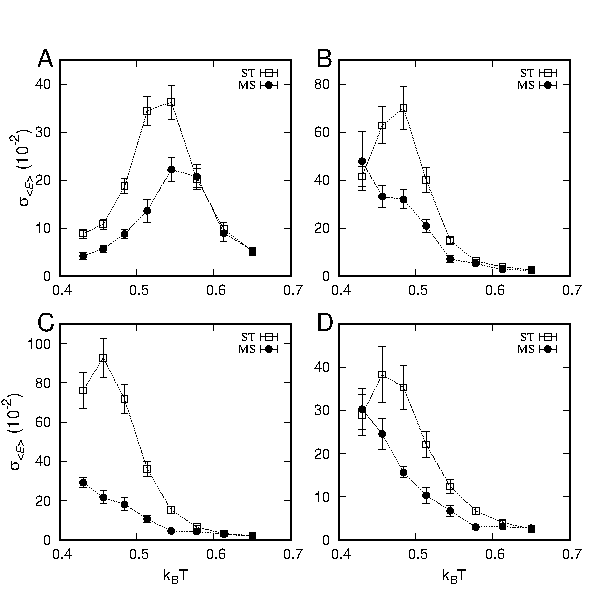
\includegraphics[width=8.0cm]{Stderr}
\caption{Computational efficiency of the multisequence and simulated tempering algorithm.}
\end{figure}


We apply the multisequence algorithm to this set of 144 sequences across a range of temperatures. Figure~2 illustrates a typical simulation carried out at the lowest temperature, $\Tlow$, which is well below the folding temperature of both A1 and N1~\cite{Holzgrafe2014,Holzgrafe2015}. From the MC evolution of the total energy $E$, sequence index j, and similarity measures $Q_A$ and $Q_B$, it is evident that visits to various sequences drive transitions into a range of structural states. For example, visits to A1 ($\mathrm{j}=1$) and N1 ($\mathrm{j}=144$) tend to coincide with visits to high-$Q_A$ and high-$Q_B$ conformations, respectively, as is necessary to generate the correct conformational ensembles for these sequences.

Sequence updates $\sbar\rightarrow\sbar'$ are carried out by picking a new sequence $\sbar'$ randomly from the entire set of allowed sequences. Therefore, a sequence update typically changes more than one amino acid position. In other words, if the step size in sequence space is $\Delta H$, then typically $\Delta H>1$. Interestingly, despite the large $\Delta H$ and low $T$, the overall (average) acceptance rate $P_\mathrm{acc}=0.xx$ for $\sbar\rightarrow\sbar'$ updates which is not unreasonably low. Higher $P_\mathrm{acc}$ can be obtained by restricting proposed moves such that $\Delta H\le\Delta H_\mathrm{max}$, as shown in Figure~3. For example, an acceptance rate close to the oft-quoted rule-of-thumb value $0.25~\cite{Gilks1996} $ is obtained with $\Delta H_\mathrm{max}=4$, and with $\Delta H_\mathrm{max} = 1$ (only point mutations), $P_\mathrm{acc}=0.xx$. For simplicity, in this work, all simulations are carried without restrictions on how new sequences $\sbar'$ are drawn. 

\begin{figure}
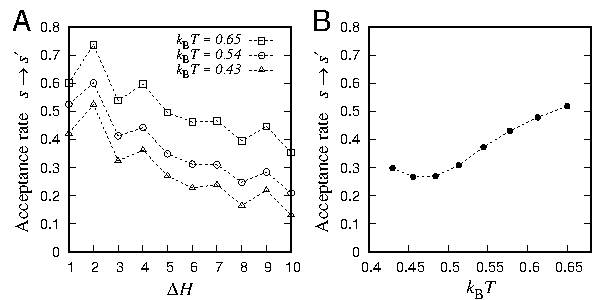
\includegraphics[width=5.8cm]{Pacc}
\caption{Averages acceptance rates $P_\mathrm{acc}$ of mutational updates $\sbar\rightarrow\sbar'$ as a function of the number of changed amino acid positions, $\Delta H$.}
\end{figure}

To assess computational efficiency, we compare with results from simulated tempering (ST) simulations carried out on 4 of the 144 sequences, namely A1 and N1 and the two sequences R1 and R2 chosen randomly at $H=4$ and $H=6$ from A1, respectively (see Table~1). While ST provides the thermodynamics of a given sequence across the 8 temperatures $T_1, ..., T_8$ in a single run, a single MS simulation provides the thermodynamics of all 144 sequences for one $T_\mathrm{i}$. We adjust the simulation lengths for ST and MS runs such that an identical number of sampled conformations are obtained for each $\sbar$ and $T_\mathrm{i}$ combination, ensuring also that similar computational resources are used for the two algorithms. 

Figure 4 shows the statistical error, $\sigma_{\left <E\right>}$, estimated for the average energy, $\left <E\right >$, for the 4 different sequences. 

\begin{figure*}
\rotatebox{0}{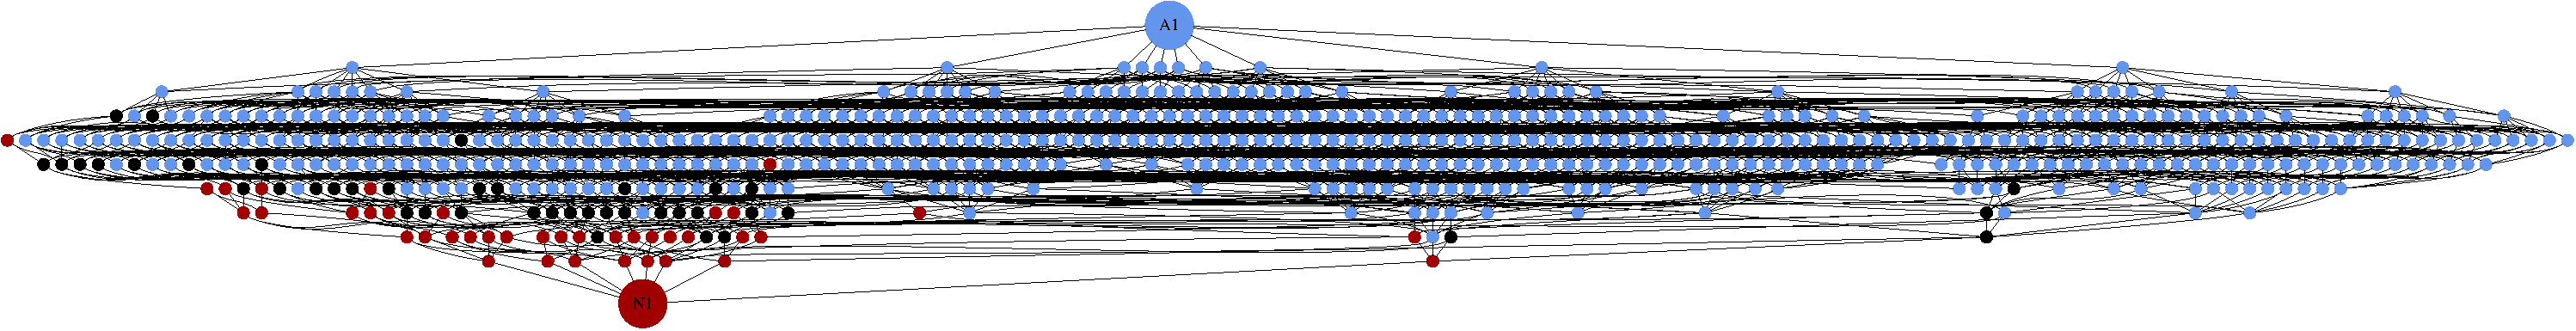
\includegraphics[width=16.6cm]{ntwk16}}\\
\rotatebox{0}{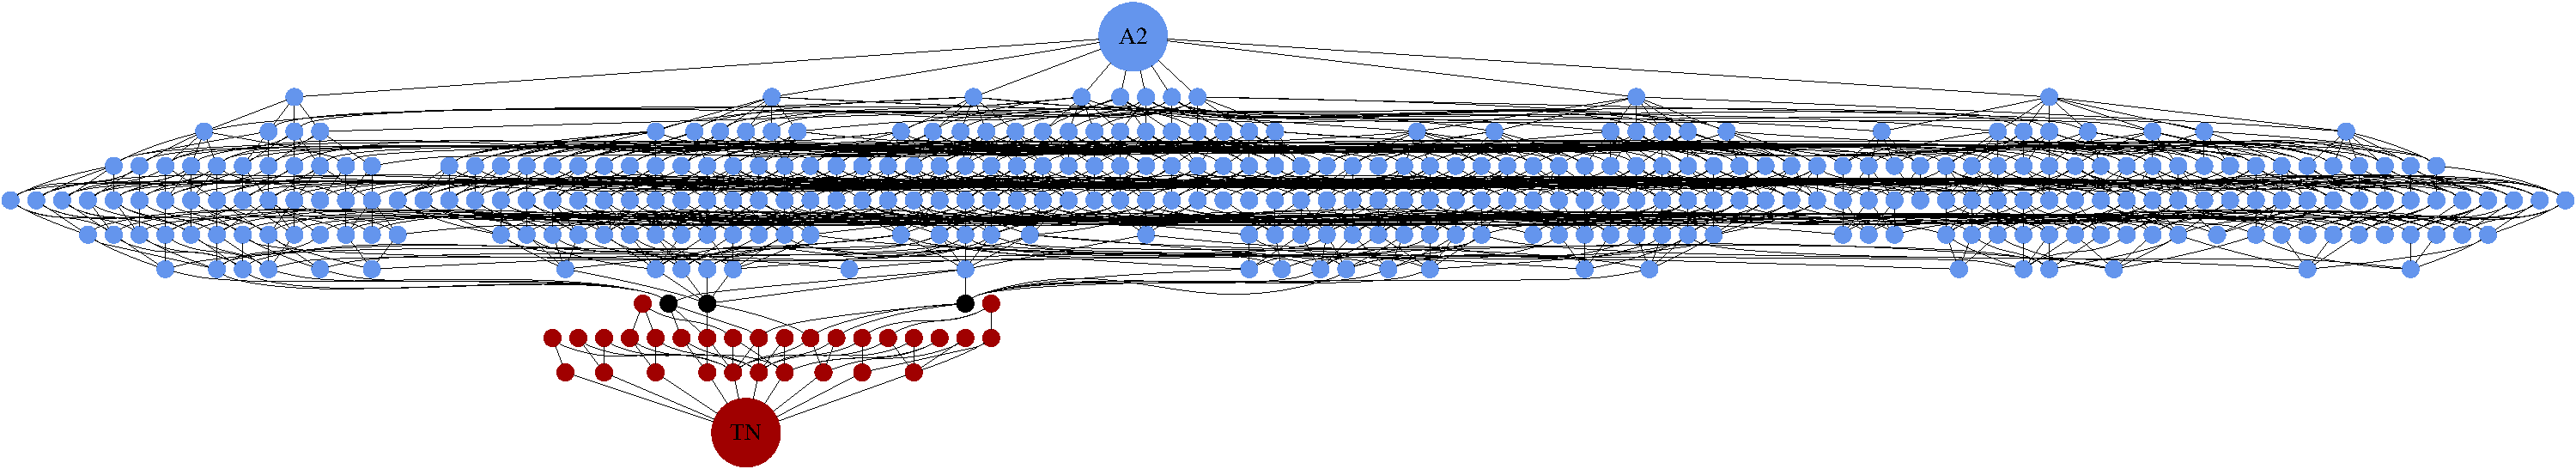
\includegraphics[width=12.6cm]{ntwk35}}
\caption{Networks of the A1-N1 (top) and A2-TN (bottom) binary sequence space. }
\end{figure*}

Hence, we conclude that in the comparison made above the computational efficiency of the MS algorithm is comparable to ST. It must be stressed, however, that while the ST simulation requires that the thermodynamic behavior is calculated at a range of temperatures, MS works well on its own directly at low temperatures. ST was introduced as an extension to the standard, fixed-$T$ Metropolis-Hastings algorithm in order to overcome the poor mixing of states at low temperatures, i.e., the tendency for the simulations at low $T$ to become trapped in local free energy minima. The MS algorithm, however, efficiently calculates the thermodynamics at low $T$'s without visits to other $T$'s. In the MS algorithm, it is visits to sequences with poor native state stability rather than high $T$'s that drive the decorrelation of generated states and escape from local traps. This way, calculation of low-$T$ thermodynamics is enhanced in MS simulations while at the same time enhancing coverage in sequence space. This makes the MS algorithm ideal for situations in which the finite-$T$ thermodynamic behavior of multiple sequences are of interest. 

\vspace{12pt}
\subsection{A1-N1 and A2-TN binary sequence spaces}
\noindent
We now apply the MS algorithm to the sets {\SI} and {\SII} which represent the full binary sequence spaces for the A1-N1 and A2-TN systems, respectively. Both sets include $2^{10}=1,024$ sequences. Using MS simulations, we determined the thermodynamic behavior at the temperatures $\TlowI$ and $\TlowII$ for the A1-N1 and A2-TN systems, respectively (see Table~1). In particular, this allow us to find the stabilities of folds IA and IB ($\PaI$ and $\PbI$) for all sequences in {\SI} and the stabilities of folds IIA and IIB ($\PaII$ and $\PbII$) for all sequences in {\SII}.


Having calculated these fold stabilities, we are in a position to determine if there are pathways in sequence space that lead to IA-IB or IIA-IIB fold changes without passing through an unstable intermediate sequence. To this end, we construct graphs in which each stable sequence is represented by a node and any two nodes are connected if their sequences differ at only one amino acid position. To determine if a sequence is stable we used the criterion $P_\mathrm{tot}>\Pcut$, where  $\Ptot = \PaI + \PbI$ and $\PaII + \PbII$ for A1-N1 and A2-AN1, respectively. The precise network obtained depends, of course, on the cut-off value of $\Pcut$. In general, a higher $\Pcut$ means a selection of more stable pathways. Fig.~5 shows the networks obtained with $\Pcut=0.50$. The number of viable mutational pathways that connect the start and end points are 516,972 between A1 and N1 and  57,912 between A2 and AN1. Because there are $10! =3,628,800$ possible mutational pathways between start and end points in both cases, these pathways represent 14.2 \% and 1.6 \% of all possible pathways in A1-N1 and A2-AN1, respectively. Hence, A1 and N1 are rather highly connected at this stability threshold. For $\Pcut=0.60$, the numbers are 104,640 pathways (2.9\%) for A1-N1 and 22,512 (0.6\%) pathways for A2-AN1. We find that there are no possible A1-to-N1 or A2-to-AN1 pathways when $\Pcut\ge0.74$ and $\Pcut\ge 0.66$, respectively. \\

\subsection{Stability properties of fold-to-fold mutational pathways}
\noindent 
An apparently general characteristic of designed and natural protein folding switching is that the stability of sequences near the switch point have reduced stability.~\cite{Bryan2010} The results from our model exhibit a similar trend. Fig.~6A and B shows the total stability $\Ptot$ at different mutational distances between start and end points. Intermediate sequences are less stable than at distances $h=0$ and $h=10$ although there are large variations as indicated by the spread between upper and lower bounds. Nonetheless, there is a clear statistical trend that sequences become less stability as more and more mutations are applied to the any of the 4 starting points. The minimum in stability occur closer to N1 or TN indicating that the all-$\alpha$ folds IA and IIA are more mutationally robust than the $\beta$-structure containing folds IB and IIB. 

\begin{figure}
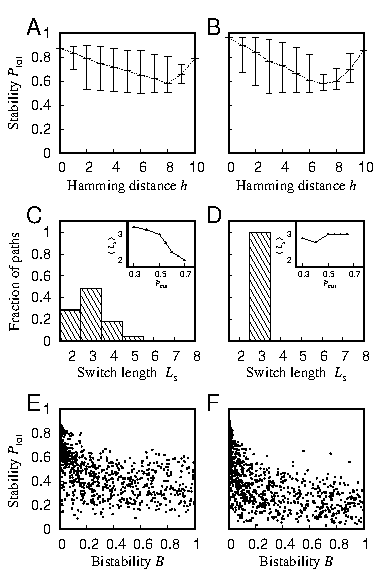
\includegraphics[width=7.8cm]{Paths}
\caption{Averages stability as a function of Hamming distance $h$. }
\end{figure}

%The smooth average stability trends in Fig.~6 might have been underpinned by individual mutational pathways that gradually shift the population between the two folds, however, this is not the case.

The smooth average stability trends in Fig.~6A and B belie the real character of the individual mutational pathways which abruptly switch from one fold to another. The switch in fold along individual pathways are typically completed in only 1-2 mutations. This can be seen from the distribution of switch lengths, $L_\mathrm{s}$, in Fig.~5C and D, taken over all pathways with $\Pcut=0.50$, where  $L_\mathrm{s} = 2$ for a switch that goes directly from a node $P_A>P_B$ to a node $P_B>P_A$ and $L_\mathrm{s} > 2$ if it also passes through one or more bistable sequences. Hence, for $\Pcut = 0.5$, it is fairly common that viable pathways pass through one or more sequences are that bistable, i.e., that have substantial populations of both folds. 

Interestingly, the passage through bistable sequences become less common for more stable pathways in the A1-TN system, as can be seen from the dependence of $\left <L_\mathrm{s}\right >$ on $\Pcut$ (see Fig.~5C(inset)). For example, for $\Pcut=0.70$, there are no viable fold switching pathways between the $\alpha$-helix and $\beta$-hairpin folds that passes through a bistable point because $\left <L_\mathrm{s}\right > =  2$. The situation for the A2-TN system is different, where $\left <L_\mathrm{s}\right >$ is relatively stable around 3. An underlying reason for this behavior is apparent by comparing the total stability and bistability of all sequences. As shown in Fig.~5E and F, there is a clear trend that sequences with high total stability do not exhibit high bistability but instead they tend to have one clearly dominant fold.

%\subsection{Super-highways in sequence space}
%
%While there are a large number possible pathways (for $\Pcut<0.60$) in both systems, there are relatively few ways to pass between the two neutral nets. For $\Pcut=0.50$, we find that there are 109 nodes in the IA neutral net and 34 nodes in the IIB neutral net through which all viable pathways pass. For $\Pcut=0.60$, these numbers reduce to 14 and 10 nodes in the IA and IIA neutral nets, respectively.
%
 
\section{Discussion}

\section{Conclusion}

\bibliography{/Users/stefan/Documents/Manuscripts/Jshort,/Users/stefan/Documents/Manuscripts/MyRefs}

\end{document}

%%%%%%%%%%%%%%%%%%%%%%%%%%%%%%%%%%%%%%%%%%%%%
%%%%%%%%%%%%%%%%%%%%%%%%%%%%%%%%%%%%%%%%%%%%%
%%%%%%%%%%%%%%%%%%%%%%%%%%%%%%%%%%%%%%%%%%%%%

\end{document}
\grid
\grid
